\documentclass[a4,11pt]{article}
\usepackage[a4paper,left=2.54cm,right=2.54cm,bottom=3cm,top=3cm,text={18cm,20cm},footskip=32pt]{geometry}
\usepackage{latexsym} 
\usepackage{amsmath}  
\usepackage{amsthm}	% per la stilizzazione dei teoremi e per gestire extra simboli matematici, size, space, font, etc..
\usepackage{amsopn}	% per stilizzazione di alcuni operatori matematici (e.g. lim e log)
\usepackage{amscd}	% per gestire frecce e circolarità tramite frecce su più livelli in un'equazione (tipo grafi)
\usepackage{amssymb} % per i simboli matematici
\usepackage{array}	% per creare e gestire array
\usepackage{actuarialsymbol} % per simboli attuariali e di matematica finanziaria 
\usepackage{mathtools} 
\usepackage{makeidx} 
\usepackage{multicol} 
\usepackage{multirow} 
\usepackage{caption} 
\usepackage{float} 
\usepackage{enumerate} 
\usepackage{graphicx}   
\usepackage{subfig} 
\usepackage{booktabs} 
\usepackage{color}  
\usepackage[english]{babel} 
\usepackage{wasysym}
\usepackage{appendix} % per inserire appendice
\usepackage{longtable}
\usepackage{hyperref}
\usepackage{collref}
\usepackage{microtype}  \graphicspath{ {Figures/}} 
\usepackage{lmodern}
\usepackage{soul}
\usepackage{bm}
\usepackage{bookmark}
\usepackage[authoryear]{natbib}
\usepackage[utf8]{inputenc}
\usepackage[T1]{fontenc}

\title{From Life Expectancy at Birth to Life Table. A Novel Approach}
\author{Andrea Nigri, Susanna Levantesi, Jos\'e Manuel Aburto}
\date{\today}

\begin{document}
	\maketitle
%\begin{abstract}
%\end{abstract}
	\bigskip
	\begin{flushleft}
		\textbf{Keywords}: Life expectancy, Forecasting, Mortality rates, Deep Neural Network.
	\end{flushleft}
%	\newpage
	
%--------------------------------------------------------------------------------------------
\section{Introduction}
%--------------------------------------------------------------------------------------------
The rise in human longevity over the last two centuries has led to a growing interest in modelling and predicting death rates and life expectancy. Reliable estimates of age-specific mortality are essential in the study of health inequalities and well-being between and within countries, however this task comes with several difficulties including lack of reliable data or stochastic variation in death counts. Because of these difficulties in several countries and sub-populations, the regularities observed in past and present trends of life expectancy have made this indicator appealing to model and predict using multiple approaches. A key advantage of modelling life expectancy at birth, or at any age, is that the predictive model deals only with a single indicator over time that summarizes the overall level of mortality, instead of modelling single time series of death rates for each age simultaneously (e.g. Lee-Carter). These approaches consider the continuous increase in life expectancy in several countries (\cite{HM}, \cite{OV2002}), how improvements have varied over time \citet{Vallin}, and the fact that females tend to reach higher ages than males (\textbf{Add Marc Luy's paper here}). However, recent patterns of stalls in mortality improvements and stagnation \cite{Ho}, or temporary reversals (\cite{aburto_16}; \cite{garcia_19}), in life expectancy observed in several countries around the globe, including the USA (\textbf{add a citation}), has made more challenging to accurately model and predict life expectancy changes.

%The frontiers of survival are raising without evidence of near deceleration and the hypothesis of an imminent boundary of human life has been repeatedly disproved by empirical evidence (\cite{HM}, \cite{OV2002}). In their influential work, Oeppen and Vaupel coined the \lq\lq best-practice life expectancy\rq\rq (BPLE) hypothesis, consisting of the linear increase of the maximum female life expectancy at a constant pace over time since 1840. Afterwards, \citet{Vallin} proposed a segmented trend line, highlighting that life expectancy cannot keep rising at the same pace. This is also evident in some countries, such as Denmark, England and the US (\cite{Aburto2018}; \cite{Hiam}; \cite{Ho}), which are experiencing decelerations in life expectancy. It is a widespread opinion that such constancy is fundamental in analyzing mortality change, thus increasing appeal on methods based on life expectancy extrapolation. Nevertheless the growing availability of reliable data, in lockstep with the improving of statistical-mathematical methods, has allowed the creation of ever-finer mortality forecasting models.

Among the mortality forecasting methods, extrapolation is the most common in demographic literature. A collection of mortality models (e.g., the Lee-Carter model \citep{LC1992} and its extensions, and the Cairns-Blake-Dowd model \citep{CBD2006}) work on the matrix of age and period death rates extrapolating the identified time-dependent and cohort-dependent parameters through a time series model.

Another approach to project mortality typically aims at forecasting the age-at-death distribution, as for example \cite{Oeppen08} and \cite{Bergeron} whom use the Lee-Carter model to project life table distribution of deaths instead of the logarithm of death rates, \cite{Pascariu19} whom introduced the forecast of the statistical moments of death distribution and \cite{BaselliniCamarda} whom propose a relational model by transforming the age axis with a smooth non-linear warping function. It is worth emphasizing that, basically, none of these models can be generalized on a wide-global dataset over age and time. Some of them adequately work in a subset of countries, some others on a subset of specific age-ranges, and so on. \cite{Cairns} proposed a set of criteria that a good mortality model should meet. They refer to good-practice guidelines, such as the consistency with historical data, the long-term dynamics biologically reasonable, but also to statistical and computational features: a good mortality model should be straightforward to implement and parsimonious. These latter features seem to advantage the univariate time series forecasting, such as the life expectancy at birth, that is easy to compute and interpret.

This last approach directly works on the univariate series of life expectancy (or other summary indicators such as lifespan disparity or entropy). The main contributions are from \cite{Lee2006}, who considers a stochastic behavior of changes in the life expectancy trend, assuming that the average changes are functions of the gap with the best-practice life expectancy (BPLE), that is the maximum life expectancy observed among national populations. Similarly, \cite{TorriVaupel12} bring forward a Geometric Brownian motion-based model, overcoming the main limitation of Lee's approach in which future life expectancy can exceed the level of BPLE. \cite{Pascariu18} take up the forecasting approaches based on the BPLE gap by using the gap between country female life expectancy and BPLE for women, and the gap with female life expectancy in the same country for men. \cite{Raftery13} introduce the idea of forecasting life expectancy using a two-sex model, developing a Bayesian hierarchical model to obtain joint probabilistic projections of life expectancy for both genders. Finally, \cite{Nigri19} propose a new approach for forecasting life expectancy and lifespan disparity based on the recurrent neural networks with a long short
term memory.

Although the use of life expectancy as a fundamental indicator of health and longevity is widespread, estimating age-specific death rates is needed for analyzing divergence in patterns of mortality at different ages, calculating other mortality indicators such as years of life lost or lifespan inequality, and for insurance pricing and pension liabilities.

The aim of this study is to formulate a model leveraging on deep learning algorithms based on neural networks to derive age-specific mortality profiles from observed or predicted life expectancy levels. Resulting estimates would be useful for guiding public health interventions, informing about age-specific mortality dynamics in contexts with deficient data collection, as well as pension and social security schemes which rely on longevity dynamics. In this article, we focus on developing the "indirect" methodology to derive age- and sex- specific death rates over time from life expectancy levels with a deep neural network framework. However, the model is flexible to be used with different summary measures such as lifespan inequality.

Demography has a long standing tradition of developing formal demographic methods and using statistical approaches to indirectly estimating indicators. According to the UN manual, the term "indirect" qualifies the demographic estimation technique that origins in the fact that such technique produces estimates of certain parameters on the basis of information that is only indirectly related to its value\footnote{The classic example is the use of the proportion of children dead among those ever borne by women aged 20-24 years to estimate the probability of dying before age 2. The observed proportion of children dead is clearly related to mortality conditions but it is not a pure mortality measure because it is affected by other non-mortality parameters.}. 
Indirect methods were developed by different systems of model life tables (\cite{UN_1955};\cite{UN_1967}; \cite{sullivan1972}); Brass’ relational model ( \cite{brass1968};\cite{brass1971}); \cite{murray2003};  \cite{wilmoth2012}; \cite{mayhew2013}.
Our work is also related to the recent improvements of forecasting techniques developed by \cite{Sevcikova} and  \cite{PascariuLL} whom, adopting a method based on the Lee-Carter model, exploit an inverse approach for converting life expectancy forecasting into age-specific death rates.

In the field of age-specific mortality forecasting from summary measures, the need for accurate and reliable estimates is yet to be met. The most recent and prominent contributions, \cite{Sevcikova} and  \cite{PascariuLL}, suffer from some structural drawbacks. Both approaches are based on the log-linear assumption, specifically, the estimation of mortality rates from life expectancy at birth can be accomplished by exploiting the regularities of age patterns of mortality. This kind of regularity might not hold for particular ages. The \cite{PascariuLL} method based on SVD estimation provides systemic divergences, underestimating from age 70 onwards and overestimating infant mortality, where the relationships between mortality rates in logarithmic scale and life expectancy at birth provide a flat correlation. 
\cite{PascariuLL} found that the optimal number of years to be used in the fitting of the model is between 30 and 35 years. On the other hand, a short period may provide hight jumps in parameter estimation, that force authors to compensate using another estimation step including the parameter noise smoothing. In this regard, a measure of the improvements provides by the smoothing is neglected.
Furthermore, some parameters have not a demographic interpretation, such as the $k$ in \cite{PascariuLL} that is just an additional step to optimize estimation. Finally, the so-called rotation of the $\beta$ parameter in the spirit of Lee and Li implies additional modeling with arbitrary thresholds into the \cite{Sevcikova} and \cite{PascariuLL} frameworks.
All these aspects might be overcome by using a fully non-parametric approach such as a deep neural network model. It provides a completely data-driven approach, allowing at investigate the hidden relationship among input-output data, by avoiding an a-priori probabilistic assumption.

%The extent of indirectness varies greatly however among procedures in term both of the reliance on models and of the number of unwanted factors that have to be allowed for the term indirect is therefore used to describe any estimation method that depends upon models or uses consistency checks, or indeed uses conventional data in an unconventional way

%For example..., \textbf{Here it would be good to include some description of indirect methods such as model life tables, look at Brass methods and the UN manual for demographic analysis.}\\

%The literature offers few research contributions in the field of deriving age-specific mortality from summary measures, and the need for accurate and reliable estimates is yet to be met. \textbf{Here I would describe that  Sevcikova and colleagues, and Marius and colleagues did in more detail, what are their assumptions, the SVD decomposition, etc, we can be a bit technical here. It is also important to mention their strengths and limitations, e.g. that they need a lot of data, the normality assumption if they don't assume poisson, etc.}  \cite{Sevcikova} which, adopting a method based on the Lee-Carter model, exploit an inverse approach for converting life expectancy forecasting into age-specific death rates using the UN’s 2014 probabilistic population projections. 

%\textbf{Here a couple of sentences highlighting our contribution to what the previous paragraph described would be useful.}
The scope of our contribution is to derive mortality surface from life expectancy at birth using a deep neural network model.
In the numerical application, we use data from Human Mortality Data Base (\cite{HM}). The model has been performed for Italy, USA, Australia, France and Japan, from 1950 to 2014 and for both sexes. Our results are then compared with the projected mortality rates obtained from the Lee-Carter model \citep{LC1992}  and the Linear Link \cite{PascariuLL} model in both versions (SVD and Poisson).
The paper is structured as follows. Section 2 describes the model based on the deep neural networks. Section 3 provides the results, while Section 4 concludes.

%--------------------------------------------------------------------------------------------
\section{Model}
%--------------------------------------------------------------------------------------------
	The term neural network (NN) originated as a mathematical model that replicates the biological neural networks of the human brain. NN architecture includes neurons, synaptic connections that link the neurons, and learning algorithms. Typically, NN is formed by three types of layers called input, hidden and output layer and each one has several neurons. Each unit in a network gets “weighted” information through synaptic links from the other connected ones and returns an output by using an activation function transforming the weighted sum of input signals. 
Aiming at creating a bridge between Deep Neural Network (DNN) and demography, we will describe the steps to obtain the target output.
Equation \ref{eq:1} describes the specific NN structure providing the logarithm of mortality surface $\mathbf{M_{(a,t)}}$ with $\mathbf{a}\in \left\{0,1,...,100\right\}$ vector of ages and $\mathbf{t}\in \left\{t_1,t_2,...,t_n\right\}$ vector of years:
\begin{equation}
log[\mathbf{M_{(a,t)}}] =
%\begin{bmatrix}
%log[\mathbf{m_{(a,t_1)}}] \\
%log[\mathbf{m_{(a,t_2)}}] \\
%log[\mathbf{m_{(a,t_3)}}]\\
%\vdots     \\
%log[\mathbf{m_{(a,t_n)}}] \\
%\end{bmatrix}
f^{k} \left(
\begin{bmatrix}
w^{(k)}_{1,1} & w^{(k)}_{1,2} &w^{(k)}_{1,3} & \cdots & w^{(k)}_{1,n} \\
w^{(k)}_{2,1} & w^{(k)}_{2,2} &w^{(k)}_{2,3} & \cdots & w^{(k)}_{2,n} \\
w^{(k)}_{3,1} & w^{(k)}_{3,2} &w^{(k)}_{3,3} & \cdots & w^{(k)}_{3,n} \\
\vdots  & \vdots  & \vdots & \ddots & \vdots  \\
w^{(k)}_{n,1} & w^{(k)}_{n,2} &w^{(k)}_{n,3} & \cdots & w^{(k)}_{n,n} \\
\end{bmatrix}
\begin{bmatrix}
H^{(k-1)}_{1} \\
H^{(k-1)}_{2} \\
H^{(k-1)}_{3} \\
\vdots     \\
H^{(k-1)}_{n} \\
\end{bmatrix}
+
\begin{bmatrix}
b^{k}_{1}\\
b^{k}_{2} \\
b^{k}_{3} \\
\vdots     \\
b^{k}_{n} \\
\end{bmatrix}
\right)
\label{eq:1}
\end{equation}
where, for a generic layer $k$, $f^{(k)}$ is the activation function, $W^{(k)}$ the weights matrix, $H^{(k)}$ the hidden layers, and $b^{(k)}$ the bias, used to control the triggering value of the activation function.
A graphical representation of the DNN model related to eq. \ref{eq:1} is given in Fig. \ref{fig:NN}.
\begin{figure}[H]
\centering
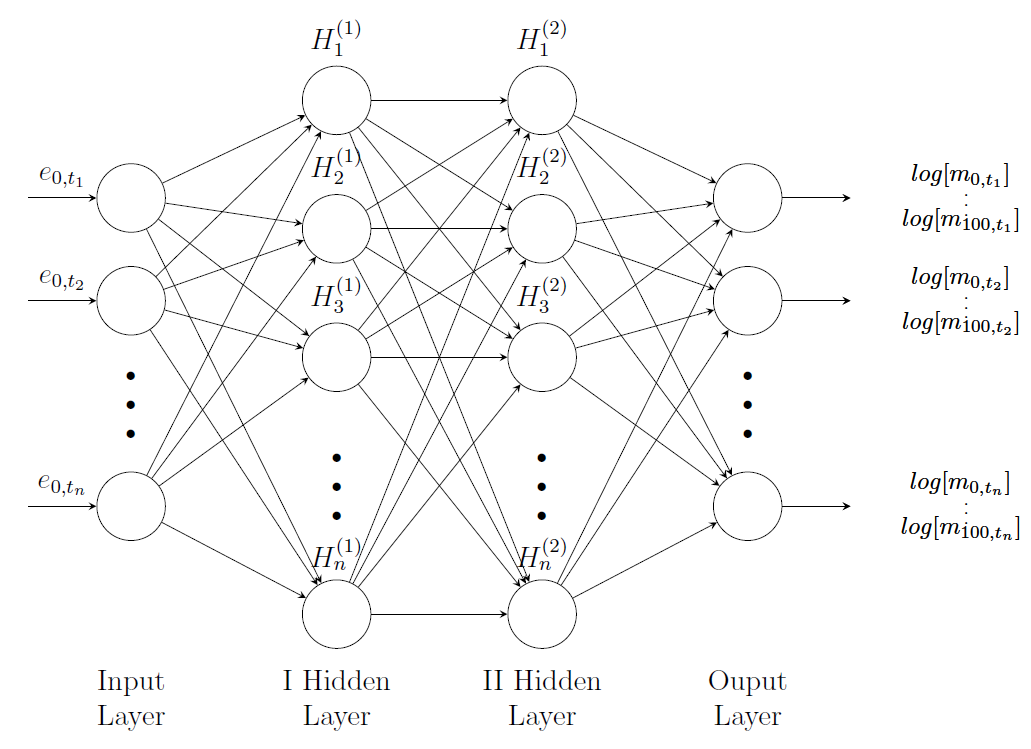
\includegraphics[width=0.8\linewidth]{NNmodel.png}
\caption{\footnotesize Graphical representation of our DNN model. Circles represent neurons, and lines synapses. Synapses take the input and multiply it by a weight (the “strength” of the input in determining the output). Neurons add the outputs from all synapses and apply an activation function.}
\label{fig:NN}
\end{figure}

In the following, we will describe the concepts from DNN in a demographic view, by defining the output as a function of the DNN structure and the input data which is the time series of life expectancy at birth. 
The theoretical relationship defining the matrix of mortality surface $log[\mathbf{M_{(a,t)}}]$ given the vector of life expectancy at birth at year $t$, and the DNN neurons processing is represented by:
\begin{equation}
log[\mathbf{M_{(a,t)}}]=f^{(k)}\big(\mathbf{W^{(k)}}\,    f^{(k-1)} \big(	\dots f^{(1)}\big(\mathbf{W^{1}\,\mathbf{e_{0,t}}}+\mathbf{b^{(1)}}\big)\dots\big)
\label{eq:2}
\end {equation}
Where $f^{(1)}\big(\mathbf{W^{1}\,\mathbf{e_{0,t}}}+\mathbf{b^{(1)}}\big) = \mathbf{H^{(1)}}$ is the first hidden layer that accepts the vector of life expectancy at birth, $\mathbf{e_{0,t}}=e_{0,t_1},e_{0,t_2},...,e_{0,t_n}$, as input.
After the estimation procedure, which implies to estimate the weights, we obtain the final output, $log[\mathbf{\hat{M}_{(a,t)}}]$, that is the mortality surface resulting from the application of the DNN parameters (weights matrix $\mathbf{\hat{W}}$ and bias $\mathbf{\hat{b}}$) obtained by the optimization procedure described in the following.\\
The estimation of the network parameters is obtained by the minimization of the overall loss function $\mathcal{L}$. We select the Mean Square Error (MSE) as loss function:
%$$\mathcal{L}(log[\mathbf{M_{(a,t)}}],log[\mathbf{\hat{M}_{(a,t)}}]) = \frac{1}{a \cdot t}\sum_{a,t}\left(log[\mathbf{M_{(a,t)}}]-log[\mathbf{\hat{M}_{(a,t)}}]\right)^2$$
$$\mathcal{L}(y,\hat{y}) = \frac{1}{n}\sum_{i=1}^{n}\left(y_i-\hat{y}_i\right)^2$$
Where $y$ is $log[\mathbf{M_{(a,t)}}]$, $\hat{y}$ is $log[\mathbf{\hat{M}_{(a,t)}}]$ and $n$ is the number of observations.
It is worth noting that the loss function implicitly involves the life expectancy function as shown in eq. \ref{eq:2}. 
To minimize the loss function, we use the Gradient Descent optimization algorithm, which iteratively moves in the direction of steepest descent as defined by the negative of the gradient.
This algorithm proceeds by minimizing $\mathcal{L}$ at each step $t$,  therefore differentiating the loss function with respect to the weights  ($\mathbf{{W}}$):
\begin{equation}
\nabla \mathcal{L}(log[\mathbf{M_{(a,t)}}],log[\mathbf{\hat{M}_{(a,t)}}])=
\begin{bmatrix}
\frac{\partial \mathcal{L}(log[\mathbf{M_{(a,t)}}],log[\mathbf{\hat{M}_{(a,t)}}])}{\partial w_{1,1}^{(1)}}\\
\frac{\partial \mathcal{L}log[\mathbf{M_{(a,t)}}],log[\mathbf{\hat{M}_{(a,t)}}])}{\partial w_{1,2}^{(1)}}\\
\frac{\partial \mathcal{L}log[\mathbf{M_{(a,t)}}],log[\mathbf{\hat{M}_{(a,t)}}])}{\partial w_{1,3}^{(1)}}\\
\vdots \\
\frac{\partial \mathcal{L}(log[\mathbf{M_{(a,t)}}],log[\mathbf{\hat{M}_{(a,t)}}])}{\partial w_{n,n}^{(k)}}\\
\end{bmatrix}
\end{equation}
For the generic weights $w_{n,n}^{(k)}$ and the $k$-th layer, the algorithm proceeds using the chain derivation rule described in the following equation:
\begin{equation}
\frac{\partial \mathcal{L}(log[\mathbf{M_{(a,t)}}],log[\mathbf{\hat{M}_{(a,t)}}])}{\partial w_{n,n}^{(k)}} =\frac{\partial \mathcal{L}(log[\mathbf{M_{(a,t)}}],log[\mathbf{\hat{M}_{(a,t)}}])}{\partial H_n^{(k)}}\,\frac{{\partial H_n^{(k)}}}{\partial z_n^{(k)}} \, \frac{\partial z_n^{(k)}}{\partial w_{n,n}^{(k)}}
 \end{equation}
where $ z_n^{(k)}=w_{n}^{(k)}\,H_{n}^{(k-1)}+b_n^{(k)}$. 

To update the weights ($\mathbf{\tilde{W}}$), the gradient of the loss function, $\nabla \mathcal{L}_t(log[\mathbf{M_{(a,t)}}],log[\mathbf{\hat{M}_{(a,t)}}])$, is multiplied by a scalar, $\eta$, often called learning rate, according to the following scheme:
%This optimization algorithm estimates the weights of the network in many iterations by minimizing $\mathcal{L}$ at each step $t$. It multiplies the gradient of the loss function by a scalar, $\eta$, often called learning rate, to update the weights according to the following scheme:
%Aiming at minimizing $\mathcal{L}$, we move in the opposite direction with respect to the gradient, updating the weights according to the following scheme:
\begin{equation}
\mathbf{\tilde{W}}=\mathbf{W}-\eta \nabla \mathcal{L}_t(log[\mathbf{M_{(a,t)}}],log[\mathbf{\hat{M}_{(a,t)}}])
\end{equation}

In a figurative way, the idea behind the gradient descent is similar to “climbing down a hill” until a global or local minimum is reached. At each update, the search moves in the opposite direction of the gradient and the learning rate $\eta$ determines the amplitude of this movement, controlling the adjustment in the weights, thus determining how fast or slow we will move towards the optimal weights.
A very large learning rate leads to a sub-optimal solution. A very small learning rate involves too many iterations to find the optimal solution. 
Then, the learning rate can be considered the most important hyper-parameter for tuning NN.

The search for the optimal parameters is then carried out through an optimization process. The NN initial weights are selected in an arbitrary (random) way so they are not optimal parameters. The iterations of the algorithm lead to the optimization of the weights and minimization of the error. 
Many algorithms have been developed to solve the problem concerning the magnitude of the gradients. We use the \textbf{RMSProp} (Root Mean Square Propagation) algorithm, proposed by \cite{hinton2012neural}, which uses a moving average of squared gradients to normalize the gradient. 
Differently from other Gradient Descent algorithms, \textbf{RMSProp} uses an adaptive learning rate instead of treating the learning rate as a hyperparameter. This means that the learning rate changes over time.\\
Thus, we will implement a preliminary fine-tuning to identify the optimal hyperparameters: epochs\footnote{The number of times algorithm explores the entire training dataset.} and neurons number for each hidden layer.

%The weights update is done at each iteration according to the following scheme:
%\begin{equation}
%\mathbf{W_{t+1}}=\mathbf{W_t}- \frac{\eta}{\sqrt{\nu_t + \epsilon}} \cdot g_t
% \end{equation}
%Where $\nu_t$ is the moving average of the squares gradient for each weight:
%\begin{equation}
%\nu_t=\rho \nu_{t-1}+(1-\rho)g^2_t \text{,}
%\end{equation}
%and $g_t$ is the gradient estimated at time $t$:
%\begin{equation}
%g_t=\frac{1}{n}\sum_{i=1}^n \nabla \mathcal{L}_t(log[\mathbf{M_{(a,t)}}],log[\mathbf{\hat{M}_{(a,t)}}])
%\label{gtadagrad}
%\end{equation}
The choices concerning the type of architecture (e.g., the number of hidden layers, units for each layer) and the hyperparameter (e.g., learning rate, activation functions, and epochs) value remains a heuristic problem for NN users: the choice often depends on the type of data and it is not an easy step. A preliminary round of hyperparameters tuning, before the testing, is highly desired.

%--------------------------------------------------------------------------------------------
\section{Other models}
%--------------------------------------------------------------------------------------------
In this paper, the performance of the proposed model is compared to the Lee-Carter, a well-established approach considered as the reference model for the forecast of mortality. 
Furthermore, nowadays in the demographic scenario the indirect estimation techniques increase their appeal, offering a remarkable forecasting accuracy in lockstep with a higher level of parsimony.
As a benchmark, we introduce a further comparison with the Linear-Link (LL) model proposed by \cite{PascariuLL}, which is one of the recent and most prominent approaches to reconstruct vital rates from the demographic summary measures. 
\subsection{Lee-Carter model}
	We present the Lee-Carter (LC) model in the Poisson framework as proposed by \cite{BDV2002}:
	%
	\begin{equation} 
	\label{eq:}
	\log{\left(\mathbf{M}_{\mathbf{a,t}}\right)}=\boldmath{\alpha}_{\text{a}}+\boldmath{\beta}_{\text{a}}\boldmath{\kappa}_{\text{t}}, 
	\end{equation}
	%
	Where $\boldmath{\alpha}_{\text{a}}$ is the age-specific parameter providing the average age profile of mortality; $\boldmath{\beta}_{\text{a}}\cdot \boldmath{\kappa}_{t}$ is the age-period term describing the mortality trends ($\boldmath{\kappa}_{\text{t}}$ is the time index 
	and $\boldmath{\beta}_{\text{a}}$ modifies the effect of $\boldmath{\kappa}_{\text{t}}$ across ages).
	The following constraints on $\boldmath{\kappa}_{\text{t}}$ and $\boldmath{\beta}_{\text{a}}$ avoid identifiability problems with the parameters:
	$$\sum_{t \in \mathcal{T}}{\boldmath{\kappa}_{t}}=0 \quad \sum_{\text{a} \in \mathcal{A}}{\beta_\text{a}}=1$$
	Mortality forecasting is obtained by modeling the time index $\boldmath{\kappa_{t}}$ by an autoregressive integrated moving average (ARIMA) process. In general, a random walk with drift properly fits the data: 
	%
	\begin{equation} 
	\label{eq:}
	\kappa_{t} = \kappa_{t-1} + \delta + \epsilon_t, \quad \epsilon_t \sim N(0, \sigma^{2}_k)
	\end{equation}
	%
	where $\delta$ is the drift parameter and $\epsilon_t$ are the error terms, normally distributed with null mean and variance $\sigma^{2}_k$.

\subsection{Linear-Link model}
Linear-Link model combines strong linear relations comparing life expectancies and age-specific death rates on a log-log scale. This method is implemented in a publicly available R package.\\
Given a life expectancy at birth level, the Linear-Link model derives mortality pattern using a linear relation. Thus, the logarithm age-specific mortality rate at time $t$ and age $\text{a}$, $m_\text{a,t}$, can be expressed as a linear function of the logarithm of life expectancy at birth, $e_{\text{0,t}}$. Formally:
	%
	\begin{equation}
	\begin{array}{l}
	\log{\left(\mathbf{M}_{\mathbf{a,t}}\right)}=\boldmath{\beta}_{\text{a}} \log(\boldmath{e}_{\text{0,t}})+\nu_{\text{a}} k+\varepsilon_{\text{a,t}} \quad \text { for } \quad \text{a} \geq 0 \\
	\\ \sum_{\text{a}=0}^{\omega} \nu_{\text{\text{a}}}=1, \quad \text {and} \quad \nu_{\text{a}} \geq 0
	\end{array}
	\end{equation}
	%
Where $\omega$ is the highest attainable age. The canonical form of the Linear-Link model is based on the least squares estimation of the slope $\beta_\text{a}$ of the linear relation between life expectancy at birth and the mortality rates over the observation time $t$. Thereby, $\beta_\text{a}$ can be regarded as an age-specific parameter and $\varepsilon_{\text{a,t}}$ denotes a set of normally distributed errors with mean zero and variance $\sigma^{2}$:
	%
	\begin{equation}
	\sum_{\text{a}}\left[\log(m_{\text{a,t}})-\beta_{\text{a}} \log(e_{\text{0,t}})\right]^{2}=\sum_{\text{a}}\left[\varepsilon_{{\text{a,t}}}\right]^{2}
	\end{equation}
	%
The model specification involves a second step estimation, by computing the singular value decomposition (SVD) of the matrix of regression residuals, obtaining the $\nu_{\text{a}}$ parameter estimation.

In order to avoid projecting age-specific noise in the jump-off life table a smoothing of the $\beta_{\text{a}}$ and $\nu_{\text{a}}$ parameters using splines is performed.
Finally, the parameter $k$ optimizes the mortality curve given in the previous step, where the difference between target life expectancy $e_{0}^{*}$ and an estimated life expectancy $e_{0}$ is below a given level, $0.001$. Where $e_{0}$ represents the level of life expectancy at birth based on the initial mortality rates $\boldmath{M}_{\mathbf{a,t}}^{*}=\exp \left\{\beta_{\text{a}}\log(e_{\text{0,t}}^{*})+\nu_{\text{a}} k\right\},$ where $\boldsymbol{k}=0$. 
Alternatively, the parameters of the model can be estimated by assuming that deaths follow a Poisson distribution. In the present analysis, we consider both canonical Linear-Link (LL) and Poisson Linear Link model (LL Pois).

%$D_{x} \sim$ Poisson $\left(E_{x} \cdot m_{x, t}\right),$ with
%$m_{x, t}=\exp \left(\beta_{x} \log e_{\theta}+\nu_{x} k\right) . \quad$ In order to use this approach death counts $\left(D_{x, t}\right)$
%and exposure data $\left(E_{x, t}\right)$ are needed. Sensitivity analysis shows that the difference

%--------------------------------------------------------------------------------------------
\section{Numerical Application}
%--------------------------------------------------------------------------------------------
In the numerical application, we consider historical mortality data collected by the \cite{HM} for Australia, Italy, Japan, Russia and USA, by gender.
We will carry out an out-of-sample test considering the same period for all countries: 1950-2014. The time frame 1950-2005 is used as train-test chunk, according to a common splitting rule 80\%-20\%. 
While, the remaining time frame 2006-2014 is used for the model validation.\\
In order to assess the models’ accuracy, we calculate the Root Mean Square Error (RMSE) and Mean Absolute Error (MAE) on the validation period 2006-2014.
\begin{equation}
	\text{MAE}: \quad \sum^{n} \frac{\mid m_{\text{a,t}} - \hat{m}_{\text{a,t}} \mid}{n},
	\end{equation}
	\begin{equation}
	\text{RMSE}: \quad \sqrt{\frac{\sum^{n} (m_{\text{a,t}} - \hat{m}_{\text{a,t}})^2}{n }}. 
\end{equation}
To be applied, our model requires that data be arranged in a $year \times age$ matrix $Y$ and vector $X$.
The $X$ vector is composed of input data, that in our case study is the time series of life expectancy at age 0. The $Y$ matrix contains the target output i.e. the mortality rates by age and year. 
The model learns the hidden pattern in the input data in a given year and gives back the output in the same year.  \\
To obtain the train-test split and avoiding the time dependence, years are randomly sampled.		
The train-test we perform is slightly different from a canonical one because the test vector is selected without using a time-dependent selection. 
Thus, in the train set, we may obtain for instance the years 1980, 1995, 1970, 2000. Conversely, in the test vector, we may observe for instance the years 2010, 1985, 1999, 1997, 1975, 2001. Clearly, the train and test set do not show a time-dependent pattern.
After the tuning procedure, for each country separately, we use the architectures with six hidden layers with five hundred neurons per layer.
We choose the Rectified Linear Unit (ReLU) activation function%\footnote{The ReLU functional form is:
%$$ReLU(x)=
%\begin{cases}
%x         & \text{se $x>0$} \\
%0           & \text{se $x\geq0$}
%\end{cases}
%$$}
 that outperformed the other functions tested for all countries. 
	
\subsection{Results}
The analysis includes numerical and graphical representation of the goodness of fit.
The following figures show the relative difference of the logarithm of central death rates between our model (DNN) and the observed values. For comparison, we also shows the relative difference for the LC model. For a given model $i$, the relative difference is defined as:
$$\Delta_{\text{a,t}}^{i}=\frac{log(\hat{m}_{\text{a,t}}^{i})-log(m_{\text{a,t}})}{log(m_{\text{a,t}})}$$
In Fig. \ref{fig:2} and \ref{fig:3} we show the heat maps (for the Italian case) which are useful for appreciating the models' differences. The DNN approach shows very high accuracy performances thanks to the deep architecture, which allows for investigating the hidden relationship between life expectancy at birth and mortality surface over time.
\begin{figure}[H]
		\centering
	\subfloat[NN]{{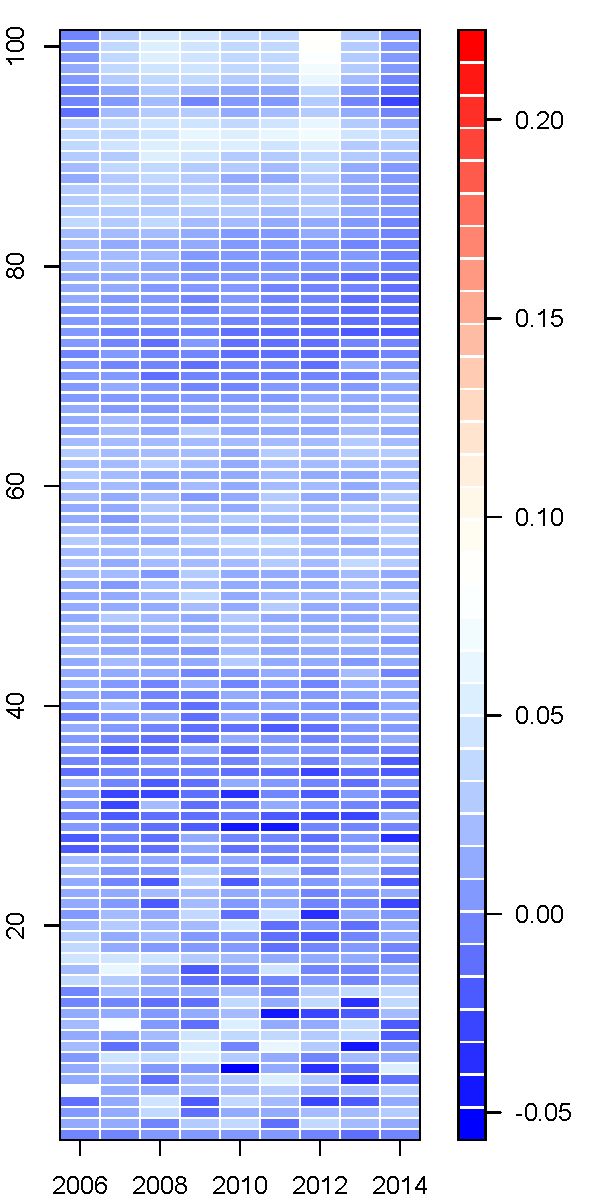
\includegraphics[width=0.25\linewidth]{ITA_F_DELTA_NN}}}
	\subfloat[LC]{{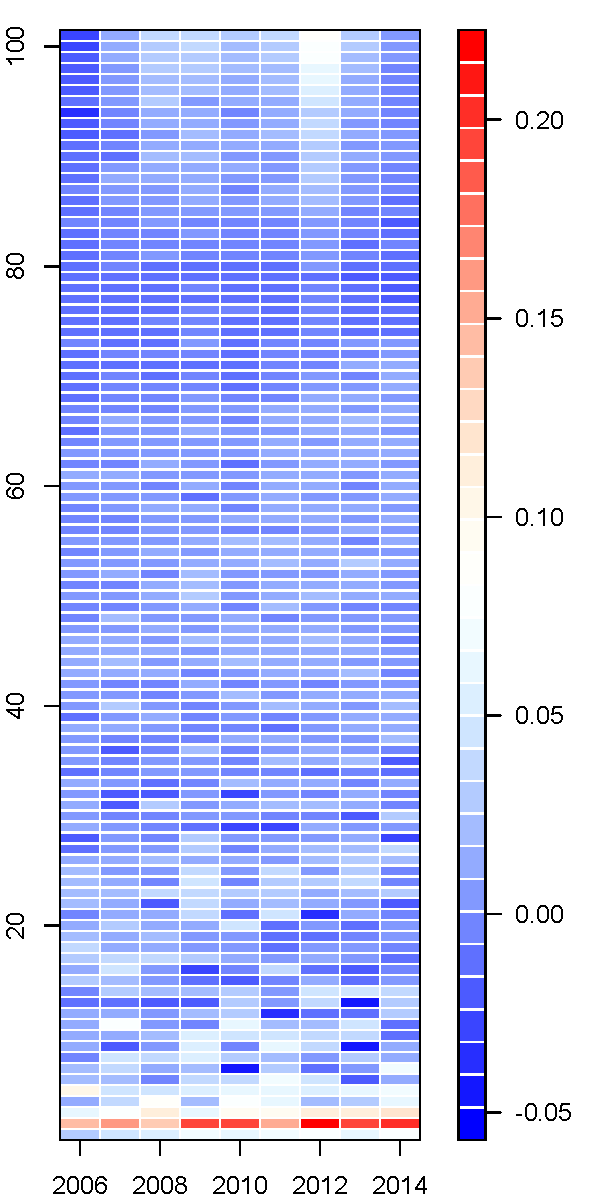
\includegraphics[width=0.25\linewidth]{ITA_F_DELTA_LC}}}
	\subfloat[LL-POIS]{{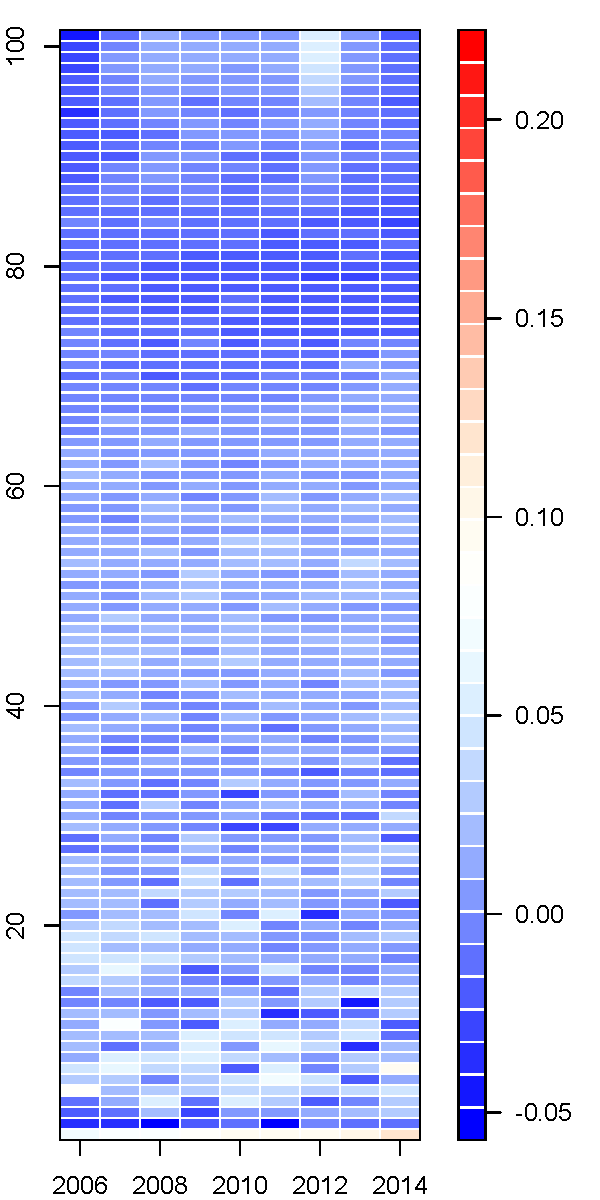
\includegraphics[width=0.25\linewidth]{ITA_F_DELTA_ll_POIS}}}
	\subfloat[LL]{{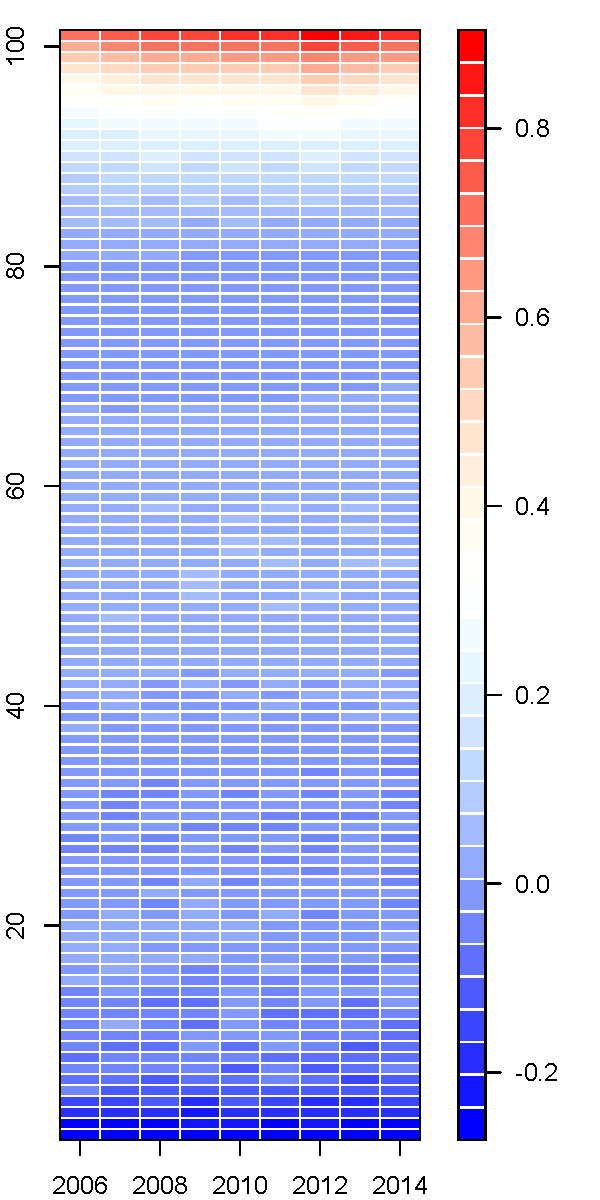
\includegraphics[width=0.25\linewidth]{ITA_F_DELTA_ll}}}
	 \caption{$\Delta_{a,t}^{i}$ - Italy, females}
	\label{fig:2}
\end{figure}

\begin{figure}[H]
		\centering
	\subfloat[NN]{{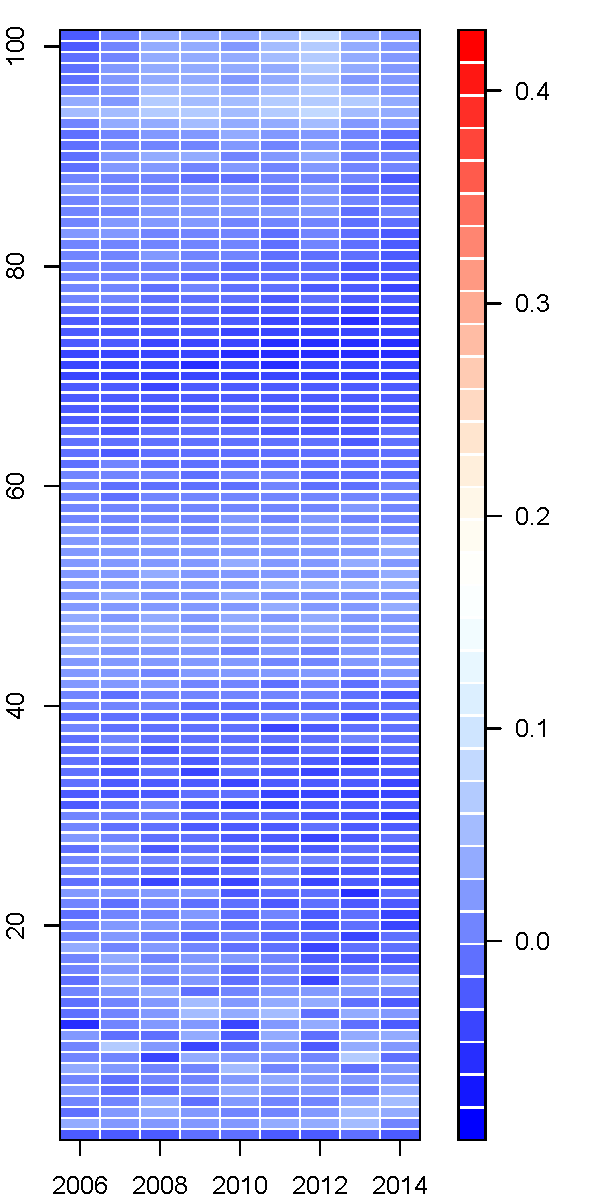
\includegraphics[width=0.25\linewidth]{ITA_M_DELTA_NN}}}
	\subfloat[LC]{{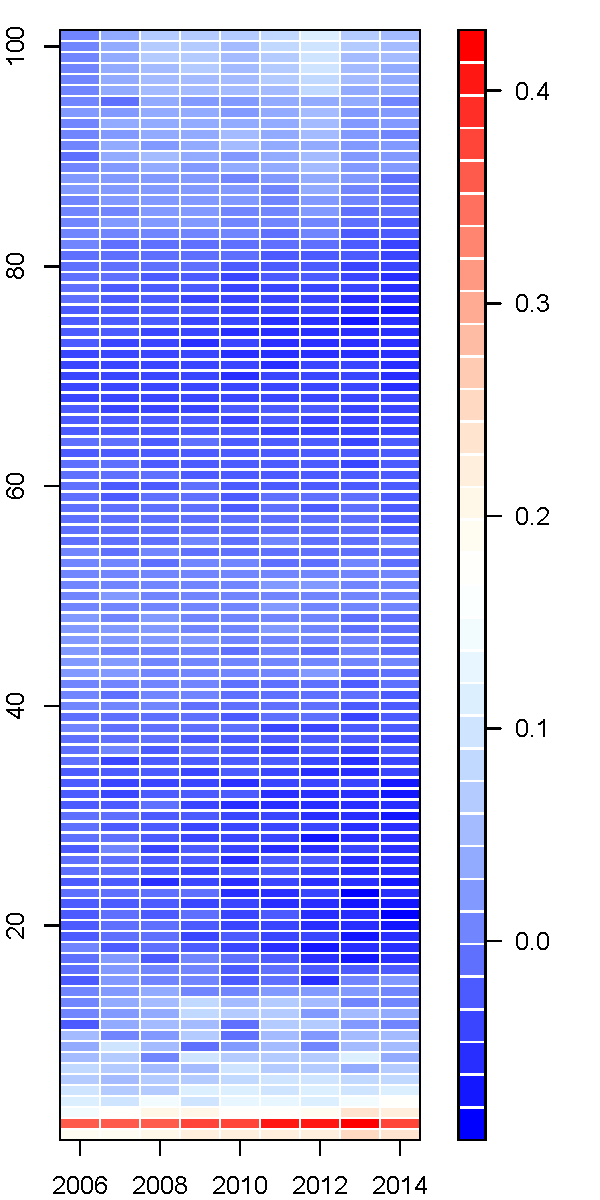
\includegraphics[width=0.25\linewidth]{ITA_M_DELTA_LC}}}
	\subfloat[LL-POIS]{{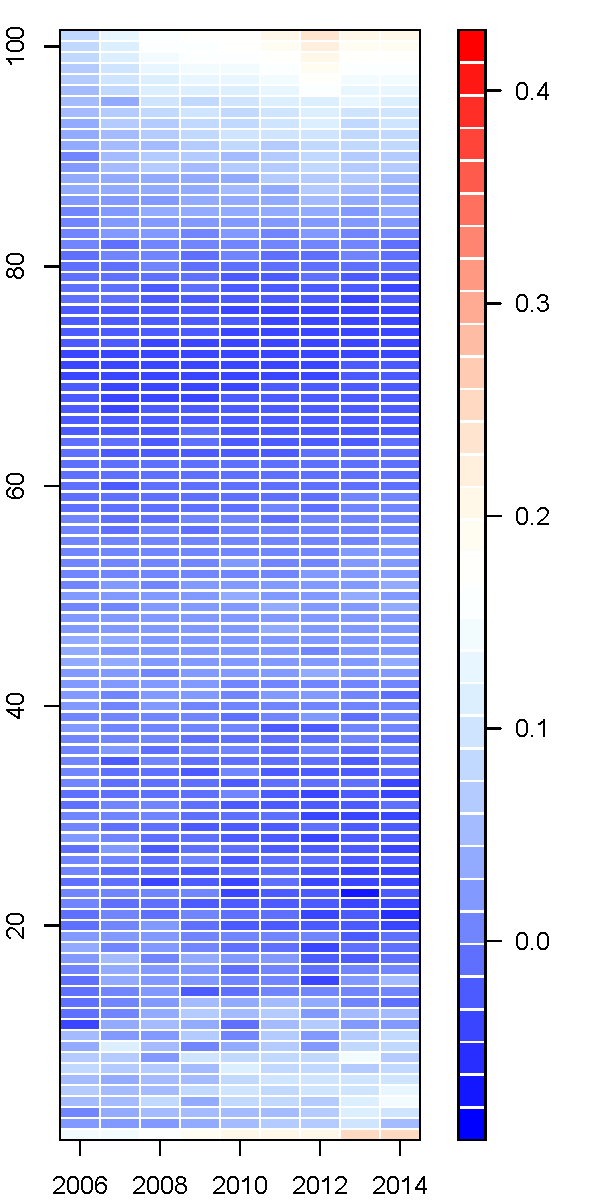
\includegraphics[width=0.25\linewidth]{ITA_M_DELTA_ll_POIS}}}
	\subfloat[LL]{{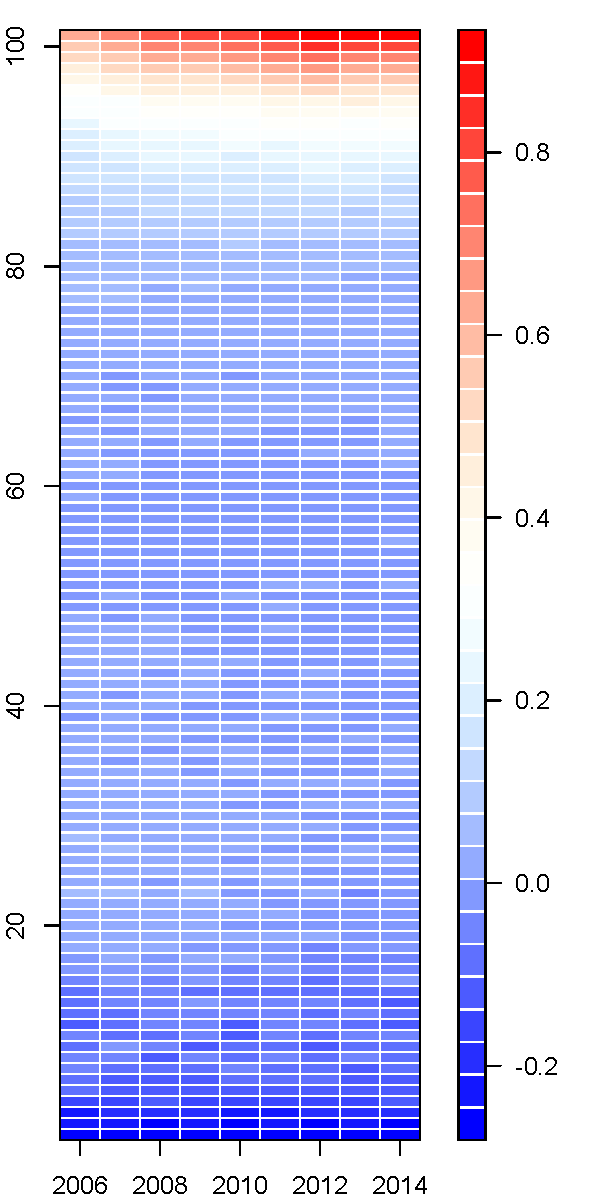
\includegraphics[width=0.25\linewidth]{ITA_M_DELTA_ll}}}
	 \caption{$\Delta_{a,t}^{i}$ - Italy, males}
	\label{fig:3}
\end{figure}
%\begin{figure}[H]
%	\centering
%	\subfloat[DNN - females]{{\includegraphics[width=0.25\linewidth]{RUS_F_DELTA_NN_}}}
%	\subfloat[LC - females]{{\includegraphics[width=0.25\linewidth]{RUS_F_DELTA_LC_}}}
%	\subfloat[DNN - males]{{\includegraphics[width=0.25\linewidth]{RUS_M_DELTA_NN_}}}
%	\subfloat[LC - males]{{\includegraphics[width=0.25\linewidth]{RUS_M_DELTA_LC_}}}
%	 \caption{$\Delta_{a,t}^{i}$ - Russia}
%	\label{fig: 4}
%\end{figure}
%\begin{figure}[H]
%		\centering
%	\subfloat[NN - females]{{\includegraphics[width=0.95\linewidth]{AUS_F_DELTA_NN}}}\\
%	\subfloat[LC - females]{{\includegraphics[width=0.95\linewidth]{AUS_F_DELTA_LC}}}\\
%	\subfloat[NN - males]{{\includegraphics[width=0.95\linewidth]{AUS_M_DELTA_NN}}}\\
%	\subfloat[LC - males]{{\includegraphics[width=0.95\linewidth]{AUS_M_DELTA_LC}}}
%	 \caption{$\Delta_{x,t}^{i}$ - Australia}
%\end{figure}
%\begin{figure}[H]
%		\centering
%	\subfloat[NN - females]{{\includegraphics[width=0.95\linewidth]{JPN_F_DELTA_NN}}}\\
%	\subfloat[LC - females]{{\includegraphics[width=0.95\linewidth]{JPN_F_DELTA_LC}}}\\
%	\subfloat[NN - males]{{\includegraphics[width=0.95\linewidth]{JPN_M_DELTA_NN}}}\\
%	\subfloat[LC - males]{{\includegraphics[width=0.95\linewidth]{JPN_M_DELTA_LC}}}
%	 \caption{$\Delta_{x,t}^{i}$ - Japan}
%\end{figure}
The logarithm of mortality surface is shown in Fig. \ref{fig:4} for the Italian males, year 2010.
\begin{figure}[H]
		\centering
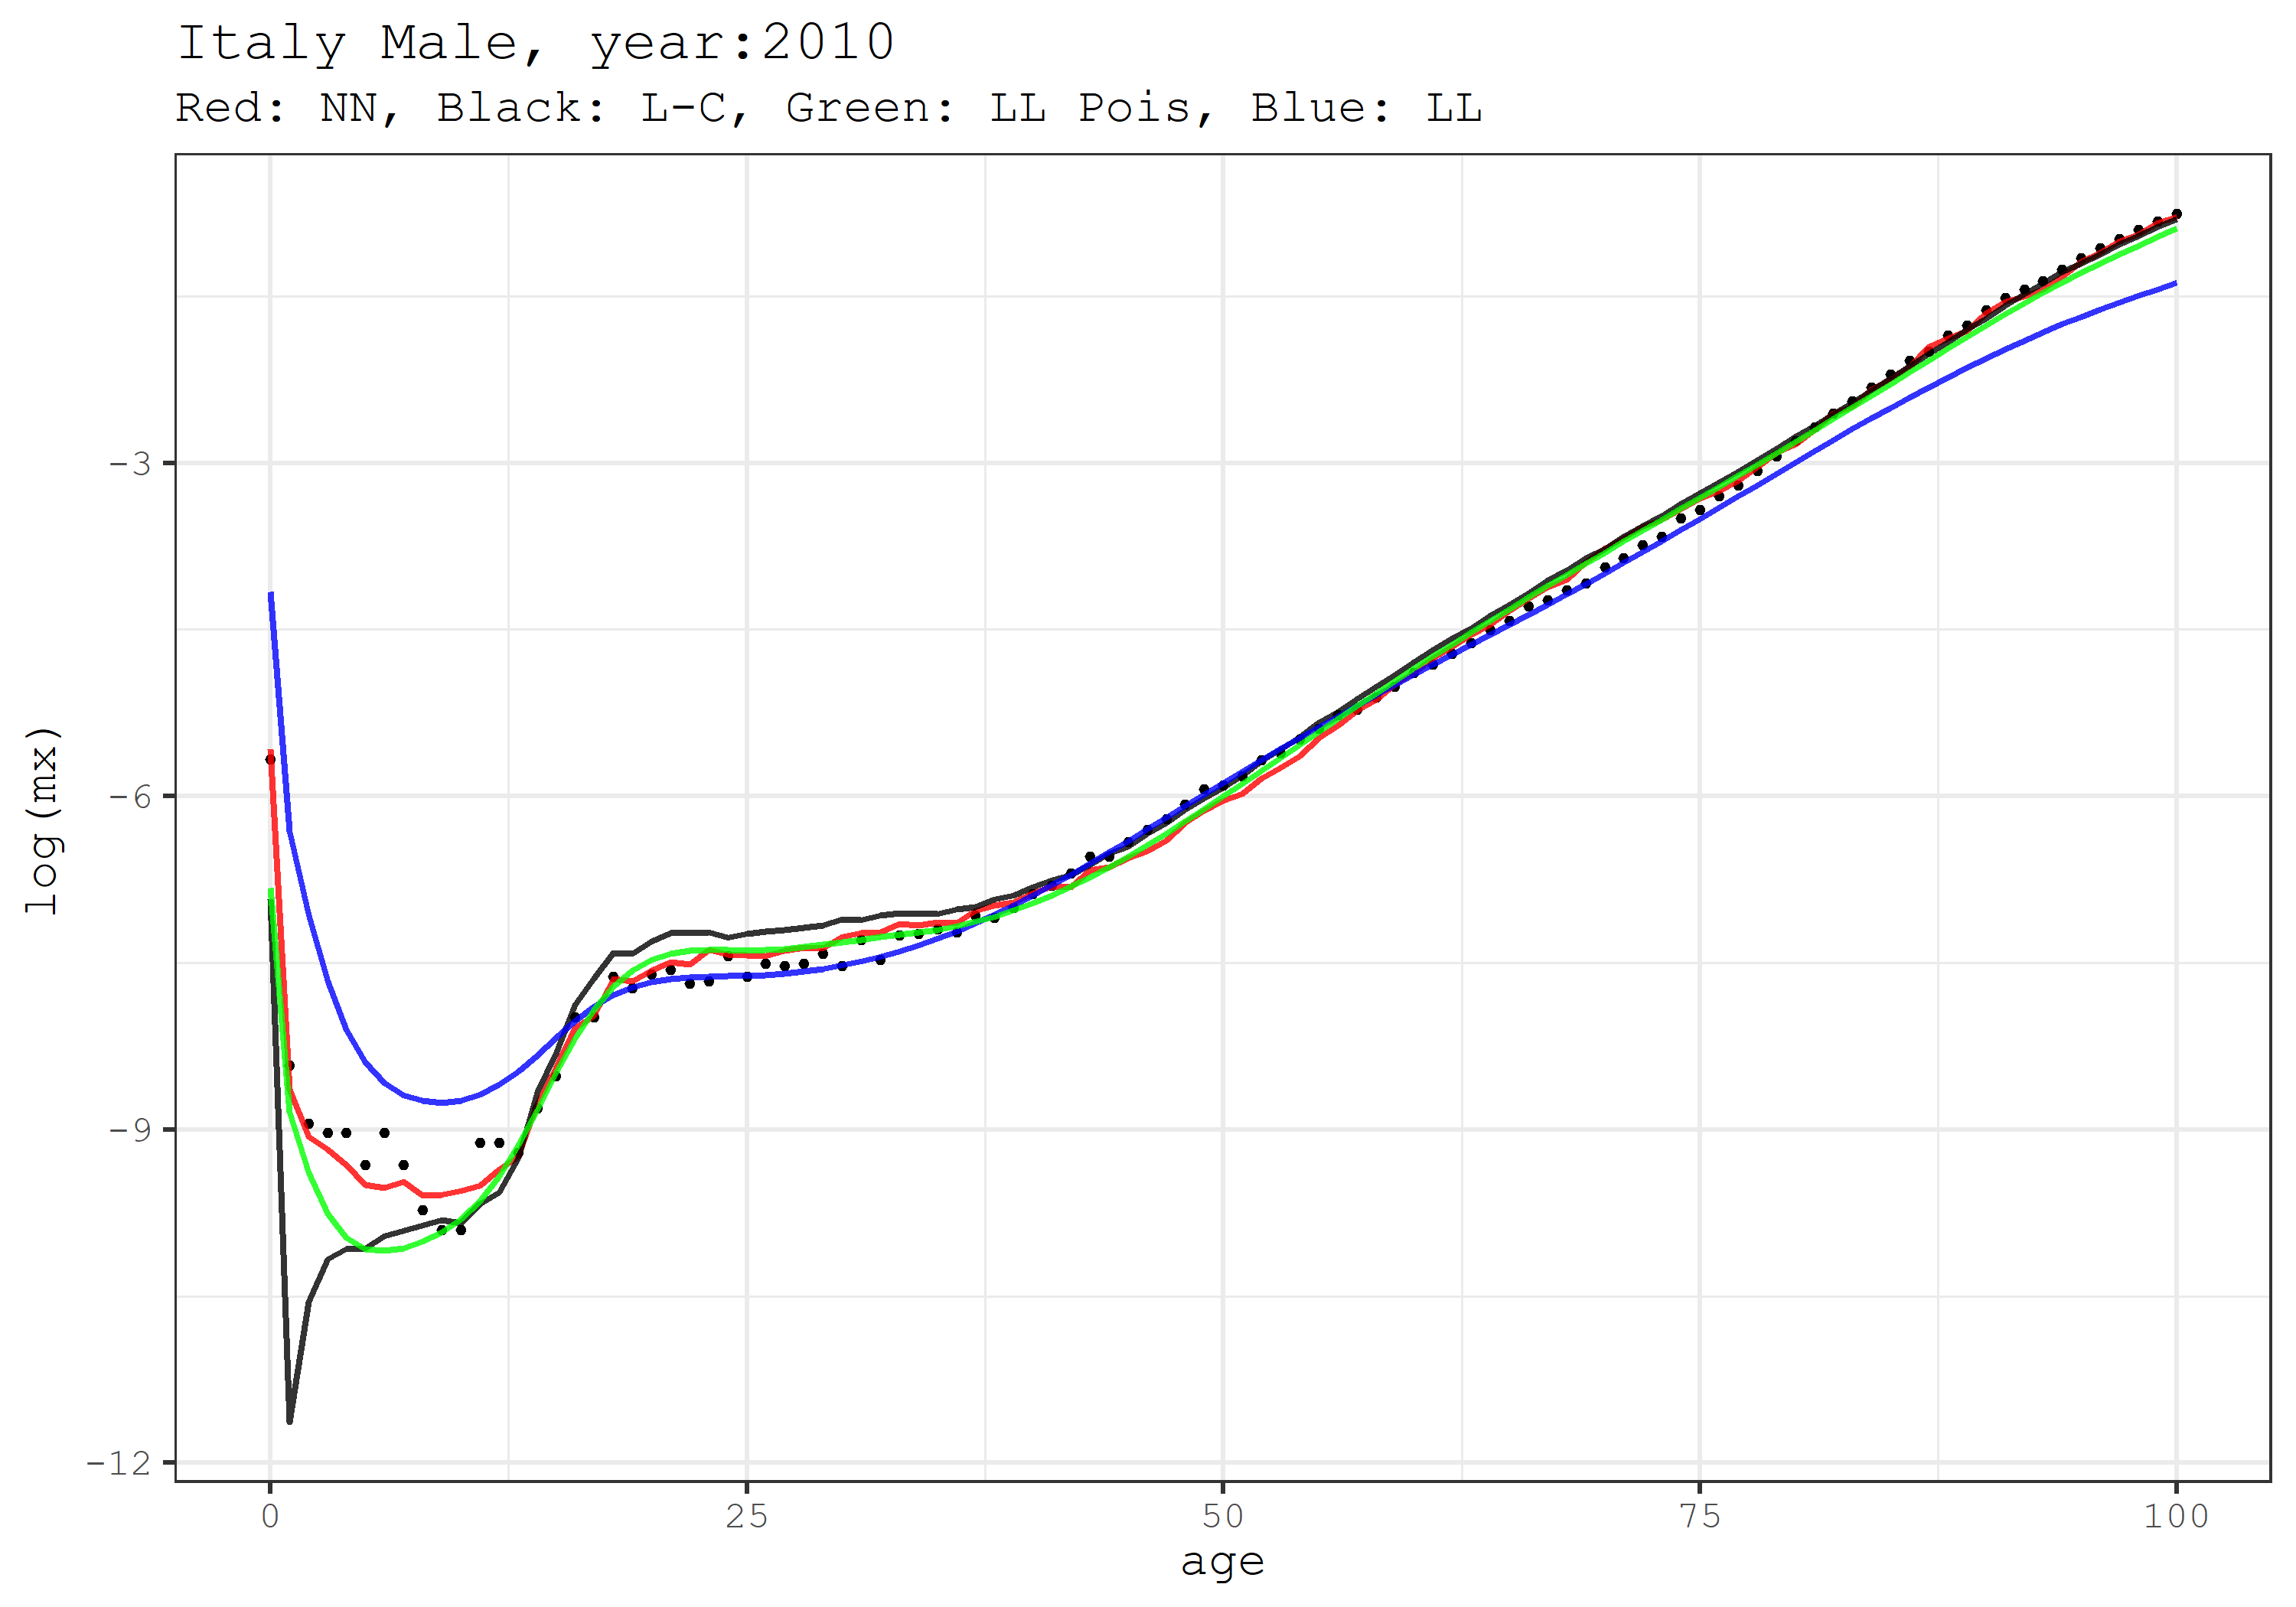
\includegraphics[width=0.75\linewidth]{m.png}
	 \caption{$log(m_a)$ - Italy, males, year 2010.}
	\label{fig:4}
\end{figure}

The values of RMSE and MAE on the validation period 2006-2014 are reported in Table \ref{tab:1}.

\begin{table}[H]
\centering
\caption{Performance of DNN the validation set for each country.}
\small
\begin{tabular}{crrrr}
			\toprule
			\textbf{Country} &  \multicolumn{2}{c}{\textbf{Female}} & \multicolumn{2}{c}{\textbf{Male}}\\
\midrule
			\textbf{\textit{Australia}}   &   \textit{MAE} & \textit{RMSE} & \textit{MAE} & \textit{RMSE}  \\
			Lee-Carter                        &   0.1381	      & 0.2080	       &   0.1734         &      0.2345  	     	\\	
               		LL                                    &   0.3101        & 0.4688         	&   0.4679         &      0.5820   		\\	
			LL Pois                             &   0.1517        & 0.2225  		&   0.1633         &      0.2164   		\\			
			DNN                                 &   \textbf{0.1295}       &\textbf{0.1984}	&   \textbf{0.1385}       &     \textbf{0.1742} 		\\
\midrule
	               \textbf{\textit{France}}      &   \textit{MAE} & \textit{RMSE} & \textit{MAE} & \textit{RMSE} \\
               		Lee-Carter                      &  0.1310    &    0.1905 	&   0.1644   &   0.2504\\	
                   	LL                                  &  0.2765    &    0.3911   	&   0.2707   &  0.3967	\\	
			LL Pois                           &	  0.1220   &    0.1593   	&   0.1047   &  0.1579	\\			
			DNN                               &   \textbf{0.1041}   &    \textbf{0.1379}   	&  \textbf{ 0.0914}   &  \textbf{0.1208}	\\
\midrule
			\textbf{\textit{Italy}}        &   \textit{MAE} & \textit{RMSE} & \textit{MAE} & \textit{RMSE}  \\
                 	Lee-Carter                      &	  0.1128      &  0.2308             &	 0.2286   &    0.4685	\\	
			LL                                  &   0.2939      &  0.4659   	    &   0.2760   &    0.4760	\\	
			LL Pois                           &	  0.1040      &  0.1586  	    &   0.1657   &    0.2667	\\			
			DNN                               & \textbf{0.0986}      &   \textbf{0.1368}   &   \textbf{0.1063}   &    \textbf{0.1403}	\\
                   	
\midrule
			\textbf{\textit{Japan}}       &   \textit{MAE} & \textit{RMSE} &  \textit{MAE} & \textit{RMSE}\\
                	Lee-Carter                       &  0.5164    &   0.7009        &	 0.1828   &   0.2886\\	
                   	LL                                   &  0.2937    &   0.4338 	&      0.2649    &   0.4490	\\	
			LL Pois                            &  0.4271    &   0.5481  	&      \textbf{0.1532}    &   \textbf{0.2200}	\\			
			DNN                                &  \textbf{0.1302}    &   \textbf{0.1771}   	&      0.1752    &   0.2338	\\
\midrule
	            	\textbf{\textit{USA}}        &   \textit{MAE} & \textit{RMSE} & \textit{MAE} & \textit{RMSE} \\
                 	Lee-Carter                      & \textbf{0.0987}  &   0.1330          &	0.10363   &    0.1375	\\	
                   	LL                                  &  0.2062  &   0.3223   	&      0.2909   &    0.3847	\\	
			LL Pois                           &	 0.1067  &   0.1535   	&      0.0969   &    0.1240	\\			
			DNN                               &  0.1000  &   \textbf{0.1276}   	&     \textbf{0.0964}   &    \textbf{0.1150}	\\
%\midrule
%	               \textbf{\textit{Russia}}      &   \textit{MAE} & \textit{RMSE} & \textit{MAE} & \textit{RMSE} \\
%               		Lee-Carter                       &  0.2229  &    0.2600 	          &   0.3444    &   0.3866\\	
%                   	LL                                  &	  \textbf{0.1685}   &   \textbf{0.2546}   	  &    \textbf{0.1838}   &   0.3007	\\	
%			LL Pois                           &   0.2538   &   0.3594   	  &   0.2211    &  0.3512	\\			
%			DNN                               &  0.1859    &   0.2598  	  &    0.1885   &  \textbf{0.2723}	\\
\bottomrule
\end{tabular}
\label{tab:1}
\end{table}	

\section{Conclusions}

Refined tools to forecast future mortality surface are becoming common among life insurers, pension plans, and social security schemes that have to manage future cash flows depending on longevity dynamics. The estimation of future mortality rates still plays a central role in the insurance industry and national public health systems. 
%From a global perspective, the forecasting of summary measures (such as life expectancy) is a common and well-established practice (\cite{Miller86};\cite{Lee93}), while the reconstruction of mortality rates from those measures is still an open debate.\\		
Our model is applied to estimating mortality rates using life expectancy or future target life expectancy. It can be also involved in projected life tables for countries with deficient data and for historical life table construction. Therefore, our model has a high degree of generalization which makes it easily applicable to different situations.

\bibliographystyle{apa}
\bibliography{bibl}

\end{document}

%\begin{thebibliography}{99}

%\bibitem[Aburto et al.(2018)]{Aburto2018}
%Aburto, J. M., Wensink, M., van Raalte, A., Lindahl-Jacobsen, R. (2018). Potential gains in life expectancy by reducing inequality of lifespans in Denmark: an international comparison and cause-of-death analysis. BMC Public Health, 18(1), 831.

%\bibitem[Basellini and Camarda(2019)]{BaselliniCamarda}
%Basellini, U., Camarda, C.G. (2019). Modelling and forecasting adult age-at-death distributions. Popul. Stud. 73 (1), 119–138.

%\bibitem[Bergeron-Boucher et al.(2017)]{Bergeron}
%Bergeron-Boucher, M.P., Canudas-Romo, V., Oeppen, J., Vaupel, J.W. (2017). Coherent forecasts of mortality with compositional data analysis. Demogr. Res. 37, 527–566. 

%\bibitem[Brouhns et al.(2002)]{BDV2002}
%Brouhns, N., M. Denuit, J. Vermunt (2002). A Poisson log-bilinear approach to the construction of projected life tables, Insurance: Mathematics and Economics, 31, 373-393.

%\bibitem[Cairns et al.(2006)]{CBD2006}
%Cairns, A.J.G., Blake, D., Dowd, K. (2006). A Two-Factor Model for Stochastic Mortality with Parameter Uncertainty: Theory and Calibration. Journal of Risk and Insurance, 73: 687--718.

%\bibitem[Cairns et al.(2008)]{Cairns}
%Cairns, A.J.G., Blake, D., Dowd, K. (2008). Modelling and management of mortality risk: a review. Scand Actuar J 2–3:79–113 Pensions Institute Discussion Paper No. PI-0814.

%\bibitem[Hiam et al.(2018)]{Hiam}
%Hiam, L., Harrison, D., McKee, M., Dorling, D. (2018). Why is life expectancy in England and Wales 'stalling'?. Journal of Epidemiology and Community Health, 72(5): 404-408.

%\bibitem[Hinton et al.(2012)]{hinton2012neural}
%Hinton, G., Srivastava, N., Swersky, K. (2012). Neural networks for machine learning lecture 6a overview of mini-batch gradient descent. 
%Lecture Notes Distributed in CSC321 of University of Toronto. 2014. Available online: \url{http://www.cs.toronto.edu/~tijmen/csc321/slides/lecture_slides_lec6.pdf}

%\bibitem[HMD(2018)]{HM}
%Human Mortality Database (2018). University of California, Berkeley (USA), and Max Planck Institute for Demographic Research (Germany). Data downloaded on 01/01/2019. \url{https://www.mortality.org}.

%\bibitem[Ho and Hendi(2018)]{Ho}
%Ho, J. Y., Hendi, A. S. (2018). Recent trends in life expectancy across high income countries: retrospective observational study. BMJ, 362, k2562.


%\bibitem[Lee(1993)]{Lee93}
%Lee, R. D. (1993). Modeling and forecasting the time series of us fertility: Age distribution, range, and ultimate level. International Journal of Forecasting 9(2), 187–202.

%\bibitem[Lee(2006)]{Lee2006}
%Lee, R.D. (2006). Mortality Forecasts and Linear Life Expectancy Trends. Perspectives on Mortality Forecasting. The Linear Rise in Life Expectancy: History and Prospects. Social Insurance Studies, 3. 

%\bibitem[Lee and Carter(1992)]{LC1992} 
%Lee, R. D., and Carter, L. R. (1992). Modeling and forecasting US mortality. Journal of the American Statistical Association, 87: 659--71.

%\bibitem[Miller(1986)]{Miller86}
%Miller, R. B. (1986). A bivariate model for total fertility rate and mean age of childbearing. Insurance: Mathematics and Economics 5(2), 133-140
	
%\bibitem[Nigri et al.(2019)]{Nigri19}
%Nigri, A., Levantesi, S., Marino, M.,  2019. Life Expectancy and Lifespan Inequality forecasting. A Deep Learning approach. (Working paper). 
		
%\bibitem[Oeppen and Vaupel(2002)]{OV2002}
%Oeppen, J., Vaupel, J.W. (2002). Broken Limits to Life Expectancy. Science, 296(5570): 1029--1031. 

%\bibitem[Oeppen(2008)]{Oeppen08}
%Oeppen, J. (2008). Coherent forecasting of multiple-decrement life tables: a test using Japanese cause of death data. In: Compositional Data Analysis Conference.
		
%\bibitem[Pascariu et al.(2019b)]{PascariuLL}
%Pascariu, M. D., Basellini, U., Aburto, J.M.,Canudas-Romo, V. The Linear Link: Deriving Age-Specific Death Rates from Life Expectancy. (\url{https://www.scor.com/sites/default/files/pascariu_-_2018_-_modelling_and_forecasting_mortality.pdf})

%\bibitem[Pascariu et al.(2018)]{Pascariu18}
%Pascariu, M. D., Canudas-Romo, V., Vaupel, J.W. (2018). The double-gap life expectancy forecasting model. Insurance: Mathematics and Economics.

%\bibitem[Pascariu et al.(2019)]{Pascariu19}
%Pascariu, M.D., Lenart, A., Canudas-Romo, V. (2019). The maximum entropy mortality model: forecasting mortality using statistical moments. Scand. Actuar. J. 2019 (8): 661-685.
		
%\bibitem[Raftery et al.(2013)]{Raftery13}
%Raftery, A. E., J. L. Chunn, P. Gerland, and H. Ševcíková (2013). Bayesian probabilistic projections of life expectancy for all countries. Demography 50 (3): 777-801.

%\bibitem[Rosenblatt(1958)]{R1958} 
%Rosenblatt, F. (1958). The Perceptron: A Probabilistic Model for Information Storage and Organization in the Brain. Psychological Review 65: 386-408.
	
%\bibitem[\v{S}ev\v{c}\'{i}kov\'{a} et al.(2016)]{Sevcikova}
%\v{S}ev\v{c}\'{i}kov\'{a}, H., N. Li, V. Kantorov\'{a}, P. Gerland, and A. E. Raftery (2016). Age-specific mortality and fertility rates for probabilistic population projections. In Dynamic demographic analysis, 285-310. Springer.


%\bibitem[Torri and Vaupel(2012)]{TorriVaupel12}
%Torri, T., Vaupel, J.W. (2012). Forecasting life expectancy in an international context. International Journal of Forecasting 28 (2): 519-531.

%\bibitem[Vallin and Mesl\'e(2009)]{Vallin} 
%Vallin, J., Mesl\'e, F. (2009). The Segmented Trend Line of Highest Life Expectancies. Population and development review, 35 (1): 159--187.
		
%\bibitem[White(2002)]{White02}
%White, K. M. (2002). Longevity advances in high-income countries, 1955-96. Population and Development Review 28 (1): 59-76.
		
%\bibitem[Wilmoth et al.(2012)]{Wilmoth}
%Wilmoth, J., Zureick, S., Canudas-Romo, V., Inoue, M., Sawyer, C. (2012). A Flexible Two-Dimensional Mortality Model for Use in Indirect Estimation
%\end{thebibliography}
